\section{Introduction}
For this homework we have been asked to solve a image classification problem choosing a dataset having at least 10 classes and 150 images for each class.
In this report I will describe the dataset, the preprocessing steps, the models used and the results obtained.

\subsection{Dataset}
The dataset I have chosen is the \href{https://www.kaggle.com/slothkong/10-monkey-species}{10 Monkey Species} dataset from Kaggle.
It is composed of 10 different classes of monkeys, each class has more than 150 images as shown in Figure~\ref{fig:dataset_distribution}.
There are almost 1400 images with resolution of 400$\times$300 px or larger and the images are in RGB format, some examples are shown in Figure~\ref{fig:dataset_examples}.

\begin{figure}[h]
    \centering
    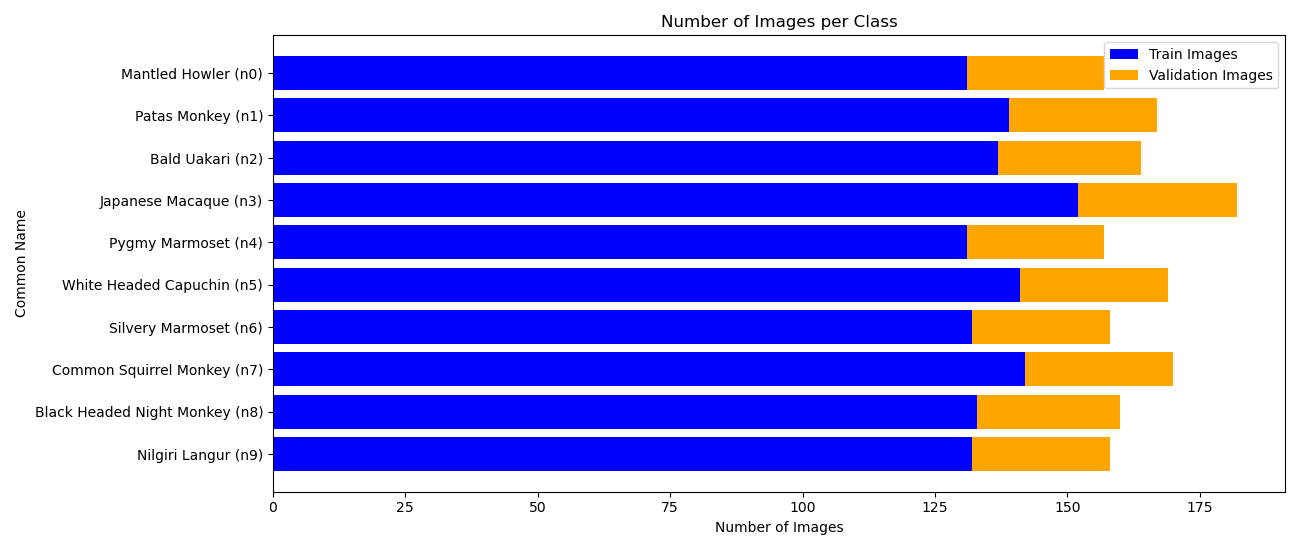
\includegraphics[width=0.9\textwidth]{../plot/monkey_labels.png}
    \caption{Dataset distribution by class}
    \label{fig:dataset_distribution}
\end{figure}


\begin{figure}[h]
    \centering
    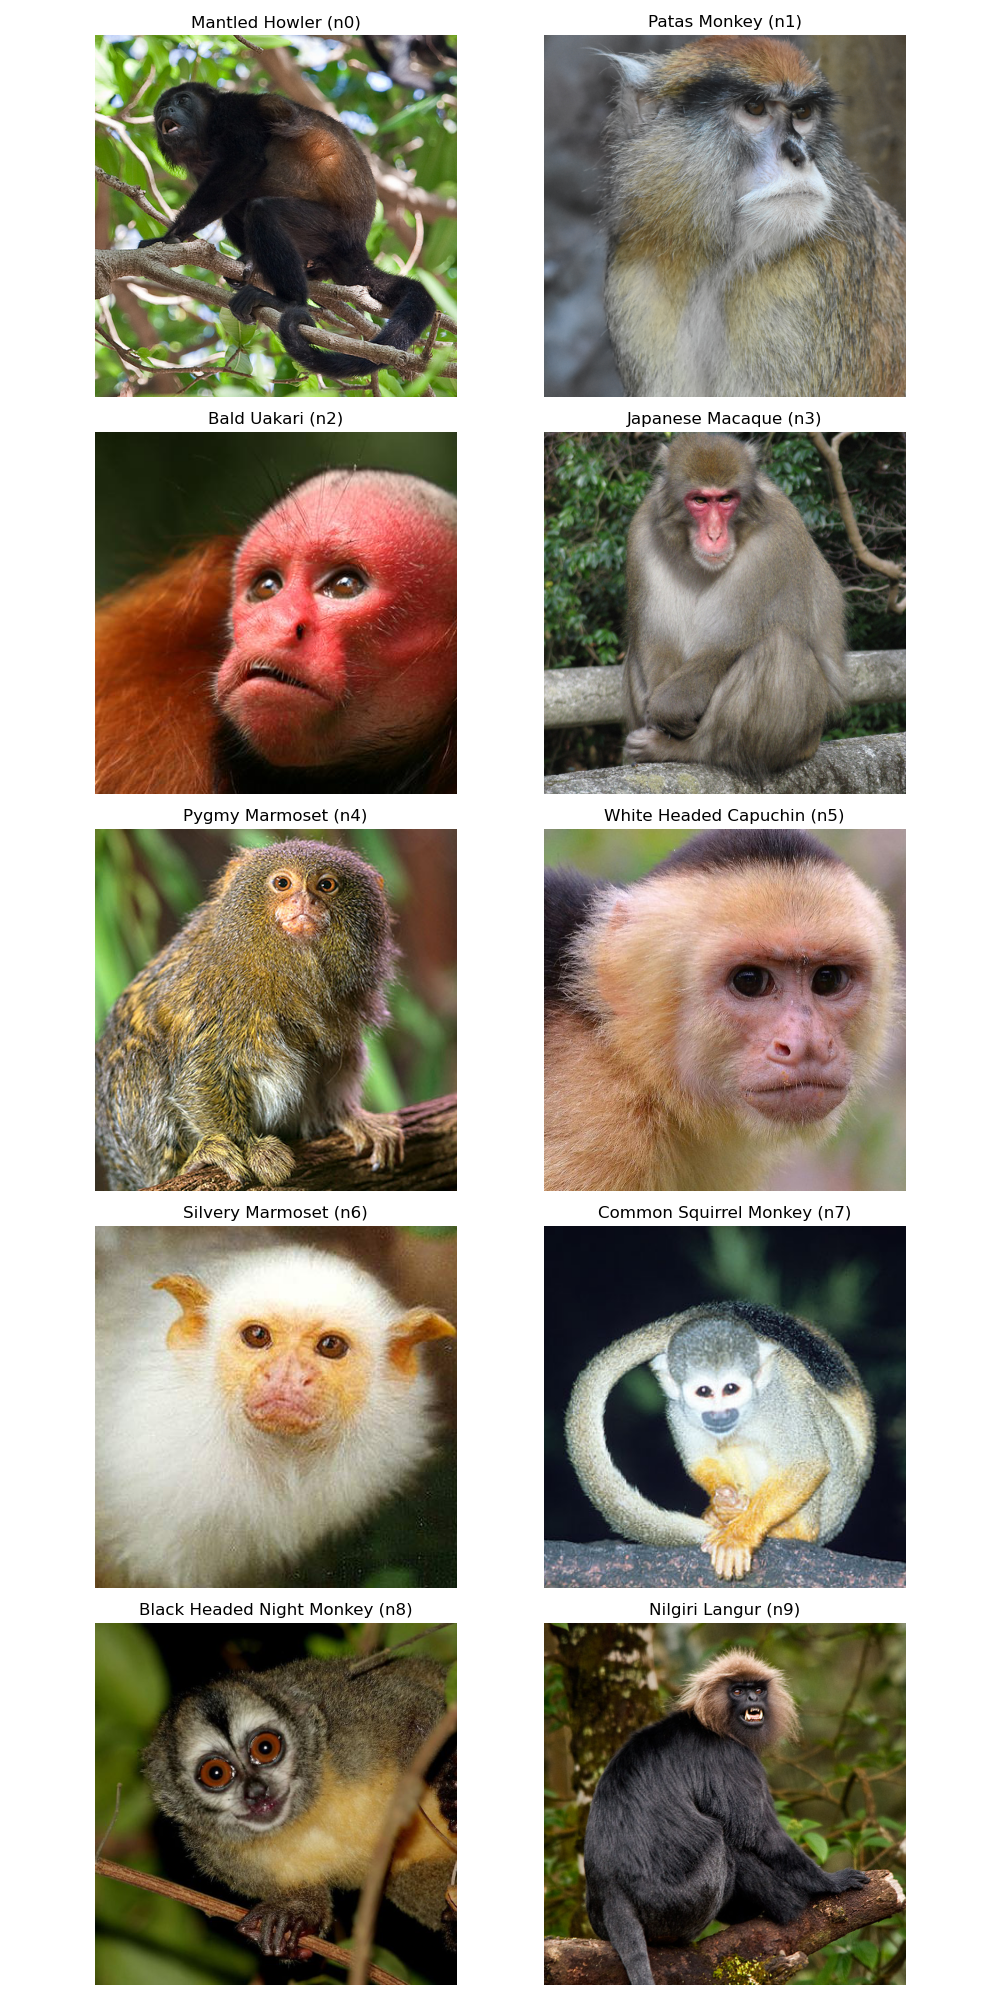
\includegraphics[height=1\textheight]{../plot/data_examples.png}
    \caption{Dataset examples}\label{fig:dataset_examples}
\end{figure}